\documentclass[14pt,portuguese]{extreport}

%Pacote para adicionar fotos
\usepackage{graphicx}
\graphicspath{ {latex_images/} }

\usepackage{indentfirst}
\usepackage[OT2,OT1]{fontenc}
\usepackage[portuguese]{babel}
\usepackage[utf8]{inputenc}

\usepackage{amsmath}

%Espaçamento duplo
\linespread{1.6}

%Comando para um trecho em Russo da biografia do Asimov
\newcommand\cyr
{
\renewcommand\rmdefault{wncyr}
\renewcommand\sfdefault{wncyss}
\renewcommand\encodingdefault{OT2}
\normalfont
\selectfont
}
\DeclareTextFontCommand{\textcyr}{\cyr}
\def\cprime{\char"7E }
\def\cdprime{\char"7F }
\def\eoborotnoye{\char’013}
\def\Eoborotnoye{\char’003}

% Titulo do livro
\title{Despertar dos Deuses} % Adiciona o T´ıtulo
\author {David Britto Jr \\ Pedro Ribeiro} % Adiciona o nome do Autor

\begin{document}

  \pagenumbering{arabic}
  
  \maketitle % Lista os tr^es dados acima como capa do livro
  
  \tableofcontents
  
  \newpage
  %Capa Livro
  \begin{figure}[h]
    \centering
    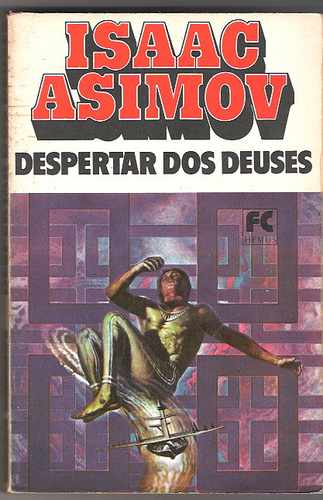
\includegraphics[width=\textwidth]{despertar_deuses_capa}
  \end{figure}
  
  \newpage
  %Asimov Sentado
  \begin{figure}[h]
    \centering
    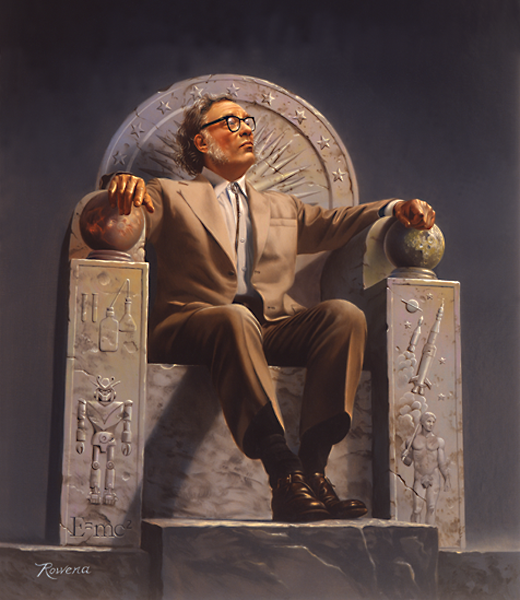
\includegraphics[width=\textwidth]{asimov_sentado}
    \caption{Isaac Asimov}
  \end{figure}

  
  \chapter{Introdução}

    \section{Apresentação da disciplina e do livro}
      
      A disciplina Engenharia e Sociedade aborda o conteúdo ético
      e moral que nós, como graduandos em engenharia, devemos
      exercitar ao seguirmos nossa profissão. Servindo assim como ponte
      entre a capacitação técnica e a sensibilidade social.
      
      Utilizaremos o livro de Isaac Asimov, O Despertar dos Deuses,
      que possui como sinopse:
      
      \begin{quotation}
	Que peripécias viverá a humanidade no futuro? Num mundo que sobreviveu a
	tremenda crise ecológica e que tem fome de energia? Quais os problemas que
	enfrentará? Do contato da Terra com um desconhecido Universo paralelo
	surgem terríveis enigmas imprevistos. Como evitar a catástrofe, que virá com a
	subversão das leis da natureza, se, contra a estupidez humana, os próprios
	deuses disputam em vão?
	
	Da Terra, à beira da tragédia, somos levados por Isaac Asimov ao estranho e
	misterioso Universo paralelo, onde seres dotados de inteligência se conduzem
	de acordo com padrão de vida completamente estranho ao nosso. E dali somos
	transferidos ao mundo Selenita, com a sua colônia humana já estabelecida e já
	desenvolvendo novas formas de convivência social. A essas situações
	fascinantes se acrescenta a emoção das paixões conflitantes de personagens
	inesquecíveis desenhados com invulgar maestria literária. Protagonistas de
	episódios cuja sucessão alucinante não esconde uma meditação profunda, em
	verdade projetada no futuro a partir da experiência crucial de nossa era.
      \end{quotation}

    \section{Objetivos do trabalho}
    
      Nesse projeto utilizamos a leitura do livro de Isaac Asimov, O
      Despertar dos Deuses, para fazermos uma analogia a respeito de
      como a humanidade em geral reagiria face a descoberta de uma
      solução energética que talvez pusesse a Terra ou até o universo em
      risco. Além do outro lado, qual grau de responsabilidade teria uma
      sociedade que solucionaria o problema da morte iminente de seu
      “Sol” colocando, conscientemente, em risco de extinção um outro
      universo. Trançamos um paralelo com a nossa formação e com o
      que significa ser um engenheiro. Além disso, a leitura do livro
      estimulou uma análise conceitual sobre personalidade do ponto de
      vista de que a psique possui três partes, e este conceito foi
      explicado ao fim.
      
    \section{Breve biografia de Isaac Asimov}
    
      Isaac Asimov nasceu em Petrovichi shtetl ou Oblast de
      Smolensk, República Soviética Russa (hoje província de Mahilou,
      Bielorrússia), filho de Anna Rachel Berman Asimov e Judah Asimov,
      um moleiro de uma família de Judeus. Em virtude das diferenças
      entre o calendário hebraico e o calendário juliano (à época ainda em
      uso na região pela Igreja Ortodoxa), bem como pela falta de
      registros, sua data de nascimento não pode ser precisada, situando-
      se entre 4 de outubro de 1919 e 2 de janeiro de 1920, sendo esta
      última considerada como a correta por Asimov, que semprecelebrou seu 
      aniversário a 2 de janeiro. A família deriva seu nome de
      {\cyr ozimiye} (ozimiye), uma palavra da língua russa que significa um
      cereal de inverno que o seu bisavô negociava, ao qual o sufixo
      paterno foi adicionado. Sua família emigrou para os Estados Unidos
      quando ele tinha só três anos de idade. Como seus pais falavam
      sempre iídiche e inglês com ele, ele nunca aprendeu russo. Enquanto
      crescia em Brooklyn, Nova Iorque, Asimov aprendeu a ler, por si
      próprio, quando tinha cinco anos e permaneceu fluente em iídiche,
      bem como em inglês. Seus pais tinham uma loja de doces, e toda a
      gente da família tinha de lá trabalhar. Revistas baratas de papel de
      polpa, chamadas pulp sobre ficção científica eram vendidas em lojas,
      e ele começou a lê-las. Por volta dos onze anos, começou a escrever
      histórias próprias e, por volta dos dezenove anos, tendo-se tornado
      fã de ficção científica, começou a vender suas histórias a revistas.
      John W. Campbell, o editor de Astounding Science Fiction,, para
      quem ele vendeu suas primeiras histórias, foi uma forte influência
      formativa e tornou-se um amigo.
      
      Asimov foi aluno das New York City Public Schools (escolas
      públicas de Nova Iorque), inclusive a Boys' High School, de Brooklyn.
      A partir daí, ele foi para a Universidade de Columbia, onde se
      graduou em 1939, depois tirando um Ph.D. em bioquímica, em 1948.
      Entretanto, passou três anos, durante a Segunda Guerra Mundial, a
      trabalhar como civil na Naval Air Experimental Station, do porto da
      Marinha em Filadélfia. Quando a guerra acabou, ele foi destacado
      para o Exército Americano, tendo só servido nove meses antes de
      ser honrosamente reformado. Durante sua breve carreira militar, ele
      ascendeu ao posto de cabo, baseado na sua habilidade para escreverà máquina, 
      e escapou por pouco de participar nos testes da bomba
      atómica em 1946 no atol de Bikini.
      
      Depois de completar seu doutorado, Asimov entrou na
      faculdade de Medicina da Universidade de Boston, com a qual
      permaneceu associado a partir daí. Depois de 1958, isto foi sem
      ensinar, já que se virou para a escrita em tempo integral (suas
      receitas da escrita já excediam as do salário acadêmico). Pertencer
      ao quadro permanente significou que ele manteve o título de
      professor associado e, em 1979, a universidade honrou sua escrita
      promovendo-o a professor catedrático de bioquímica. Os arquivos
      pessoais de Asimov, a partir de 1965, estão arquivados na Mugar
      Memorial Library da universidade, doados por ele a pedido do
      curador, Howard Gottlieb. A colecção preenche 464 caixas em 71
      metros de prateleira.
      
      Asimov casou-se com Gertrude Blugerman (Canadá, 1917 —
      Boston, 1990), em 26 de julho de 1942. Tiveram duas crianças, David
      (n. 1951) e Robyn Joan (n. 1955). Depois da separação, em 1970, ele
      e Gertrude divorciaram-se em 1973, e Asimov casou-se com Janet O.
      Jeppson mais tarde, no mesmo ano.
      
      Asimov era um claustrofilo; gostava de espaços pequenos
      fechados. No primeiro volume da sua autobiografia, ele conta um
      desejo infantil de possuir uma banca de jornais numa estação de
      metrô de Nova Iorque, dentro da qual ele se fecharia e escutaria o
      ruído dos carros enquanto lia.
      
      Asimov tinha medo de voar, só o tendo feito duas vezes na vida
      inteira (uma vez, durante seu trabalho na Naval Air Experimental
      Station, e outra, na volta para casa da base militar de Oahu, em1946). 
      Raramente viajava grandes distâncias, em parte por causa de
      sua aversão a voar, adicionada às dificuldades logísticas de viajar
      longas distâncias. Esta fobia influenciou várias das suas obras de
      ficção, como as histórias de mistério de Wendell Urth e as novelas
      sobre robôs de Elijah Baley. Nos seus últimos anos, ele gostava de
      viajar em navios de cruzeiro e, em várias ocasiões, ele fez parte do
      "entretenimento" no cruzeiro, dando palestras baseadas em ciência,
      em navios, como os RMS Queen Elizabeth 2. Asimov sabia entreter
      muitíssimo bem, era prolífico e procurado como discursador. Seu
      sentido de tempo era fantástico; ele nunca olhava para um relógio,
      mas invariavelmente falava precisamente o tempo combinado.
      
      Asimov era um participante habitual em convenções de ficção
      científica, onde ficava amável e disponível para conversa. Ele
      respondia pacientemente a dezenas de milhares de perguntas e
      outro tipo de correio com postais, e gostava de dar autógrafos.
      Embora gostasse de mostrar seu talento, raramente parecia levar-se
      a si próprio demasiadamente a sério.
      
      Ele era de altura mediana, forte, com bigode e um óbvio
      sotaque de judeus do Brooklyn. Seu físico era bastante limitado. Ele
      nunca aprendeu a nadar ou andar de bicicleta; no entanto, aprendeu
      a conduzir um carro, depois de se mudar para Boston. No seu livro
      de humor, Asimov Laughs Again, ele descreve a condução em Boston
      como "anarquia sobre rodas".
      
      Ele demonstrou seu amor por conduzir, em seu conto de ficção
      científica, Sally, sobre carros-robôs. Um leitor atento reparará que
      ele faz uma descrição detalhada de um dos carros a que chama
      'Giuseppe', de Milão - o que significa que Giuseppe era um AlfaRomeo. 
      Asimov não especificou nenhum outro tipo de veículo em
      nenhuma das suas histórias, o que levou muitos fãs a considerarem
      que ele foi contratado por aquela marca de automóvel.
      
      Os interesses variados de Asimov incluíram, nos seus anos
      tardios, sua participação em organizações devotadas à opereta de
      Gilbert and Sullivan e em The Wolfe Pack, um grupo de seguidores
      dos mistérios de Nero Wolfe, escritos por Rex Stout. Ele era um
      membro proeminente da Baker Street Irregulars, a mais importante
      sociedade sobre Sherlock Holmes. De 1985 até sua morte em 1992,
      ele foi presidente da American Humanist Association; seu sucessor
      foi o amigo e congênere escritor, Kurt Vonnegut. Ele também era um
      amigo próximo do criador de Star Trek, Gene Roddenberry, e foram-
      lhe dados créditos em Star Trek: The Motion Picture, pelos conselhos
      que deu durante a produção.
      
      Asimov morreu em 6 de abril de 1992 em Nova Iorque. Foi
      cremado e suas cinzas foram espalhadas. Ele deixou sua segunda
      mulher, Janet, e as crianças do primeiro casamento. Dez anos depois
      da sua morte, a edição da autobiografia de Asimov, It's Been a Good
      Life, revelou que sua morte foi causada por AIDS; ele
      contraiu o vírus HIV através de uma transfusão de sangue recebida
      durante a operação de bypass em Dezembro de 1983. A causa
      específica da morte foi falha cardíaca e renal, como complicações da
      infecção com o vírus da AIDS.
      
      Janet Asimov escreveu no epílogo de It's Been a Good Life que
      Asimov o teria querido tornar público, mas seus médicos
      convenceram-no a permanecer em silêncio, avisando que o
      preconceito anti-AIDS estender-se-ia a seus familiares. A família de
      Asimov considerou divulgar sua doença antes de ele morrer, mas a
      controvérsia que ocorreu, quando Arthur Ashe divulgou que ele
      tinha AIDS, convenceu-os do contrário. Dez anos mais tarde, depois
      da morte dos médicos de Asimov, Janet e Robyn concordaram que a
      situação em relação à AIDS podia ser levada a público.
      
  \chapter{Resumo}

    \section{Contra a estupidez...}
    
	O livro, curiosamente, começa no capítulo 6. Asimov optou por não começar no capítulo 1, pois ele vai apresentando os personagens da trama atual, o doutor Peter Lamont e o linguista Myron Bronowski, 
	ao mesmo tempo que ele faz um flashback sobre a criação da Bomba de Elétrons. Asimov faz isso da forma que, os primeiros capítulos falam sobre Frederick 
	Hallam e a descoberta/criação da Bomba de Elétrons, e são intercalados por fragmentos do capítulo 6, onde Lamont e Bronowski estão discutindo uma reunião de Lamont com Hallam.
	
	A primeira parte do livro fala do conflito de Lamont e Hallam, que deu início quando Lamont entrevista Hallam com intuíto de escrever a história da criação da Bomba de Elétrons. 
	Esse conflito resultou na pesquisa de Lamont sobre o efeito colateral da Bomba de Elétrons que causaria a destruição do sistema solar. 
	Entretanto, Hallam destruiu sua credibilidade e as hipóteses levantadas por Lamont não foram aceitas, e embora estivesse correto, nada pode fazer para impedir a destruição da Terra. 
	Essa parte do livro também foca na criação e funcionamento da Bomba de Elétrons e nos primeiros conceitos de física para-teórica.

	\subsection {Capítulo 6}

	  O capítulo 6 começa com uma diálogo entre Lamont e Bronowski. 
	  Lamont conta para Bronowski que a entrevista que ele acabou de ter com Hallam foi um fiasco maior do que a primeira. 
	  Bronowski comenta que Lamont já esperava esse resultado, conforme ele mesmo havia dito anteriormente. 
	  Lamont então segue dizendo que ele depende agora do trabalho de Bronowski, que responde dizendo que seu trabalho de enteder os para-homens é difícil, 
	  já que é um povo mais inteligente que os seres humanos, e que as vezes se pergunta se é mesmo possível inteligencias diferentes se comunicarem de alguma forma. 
	  Lamont diz que sente isso quando está explicando alguma coisa para Hallam, menosprezando a capacidade de entendimento dele.

	\subsection{Capítulo 1}

	  O capítulo 1 começa contando a história da criação da Bomba de Elétrons. Isso se passa 30 anos antes dos eventes atuais, quando o Frederick Hallam era um radioquímico recém graduado como doutor. 
	  O livro apresenta então a primeira evidência da Bomba de Elétrons, o frasco tungstênio que se encontrava na mesa de Hallam. Esse frasco não era dele, ela foi deixada por um antigo empregado e 
	  não tinha mais uso para ninguém. 
	  
	  No dia 3 de Outubro de 2070, Hallam chega no trabalho e nota que seu frasco de tungstênio havia sido alterado. Ele não tinha nenhum uso para o tungstênio, mas odiava que mexessem em sua mesa.
	  Ele acusa Denison, que nega e disparava: ``Como você saberia?``, dando a entender que Hallam não tinha inteligência o suficiente para identificar uma diferença no frasco. Denison era 
	  tão novo quanto Hallam, e era a estrela do departamento. Hallam, enfurecido, estava determinado a provar que o conteúdo não era tungstênio.
	  
	  Hallam levou o frasco para o departamento do espectrômetro de massa, a fim de descobrir qual era aquela substância. Sendo um radioquímico, Hallam conhecia as pessoas daquele departamento, e ele era 
	  insistente. Após os testes, confirmou-se que o conteúdo do frasco não era tungstênio. Entretanto, também não sabiam o que era, pois a razão carga-massa estava muito alta. 
	  Isso não foi o suficiente para Hallam, pois não bastava identificar que o frasco foi alterado, ele precisava saber o que era. Hallam mandou o técnico descobrir a carga nuclear da substância desconhecida.
	  
	  Alguns dias depois, o técnico voltou a sala de Hallam, dizendo que encontrou a carga nuclear da substância, mas estava errada. O resultado era que a substância era Plutônio-186. 
	  Este isótopo de Plutônio é impossível de existir, com 94 prótons e 92 neutrôns. Então Hallam pensou, o tungstênio que foi trocado era tungstênio-186, com 74 prótons e 112 neutrôns. 
	  Ele cogitou a possibilidade de alguma coisa ter transformado 20 neutrôns em 20 prótons. Para adicionar ainda mais incerteza no resultado obtido, a substância era estável. 
	  Esse resultado também não era satisfatório para Hallam, pois plutônio-186 é um elemento impossível.
	  
	  Duas semanas depois, Hallam descobre que o elemento estava radioativo. Nesse momento, ele já dedicava todo seu foco para resolver esse mistério, deixando de lado projetos mais importantes que ele 
	  tinha para fazer. 
	  
	  Hallam entra em contato com G. C. Kantrowitsch, que estava em seu último ano de uma carreira brilhante. Sua ajuda era difícil de conseguir, mas uma vez que obtida, o projeto 
	  avançava com grande velocidade. Dois dias depois, Kantrowitsch foi a sala de Hallam, visivelmente animado, informar que o elemento estava emitindo pósitrons, os mais energéticos pósitrons que 
	  ele já havia visto, e que a radioatividade do elemento estava aumentando a cada medida que ele fazia.

	\subsection{Capitulo 6 (continuação)}

	  Lamont explica para Bronowski que ele já considerou Hallam um grande homem, mas hoje ele o vê como um vilão, que reescreveu a história da Bomba de Elétrons para seu ganho. 
	  Lamont o descreve como um pigmeu com um único talento, de convencer as pessoas que ele é um gigante.

	\subsection{Capítulo 2}

	  Lamont tinha 2 anos de idade quando Hallam desconfiou do tungstênio alterado pela primeira vez. Quando ele tinha 25 anos de idade, se juntou a Primeira Estação de Bombeamento, 
	  logo depois que ele se tornou doutor em Física. Foi uma grande conquista para uma pessoa tão jovem. Ele foi empregado para lidar com problemas da mais alta abstração teórica, 
	  e ainda assim ele se viu fascinado pela história do desenvolvimento da Bomba de Elétrons. Ela nunca havia sido escrita por alguém que entendesse completamente os princípios 
	  teóricos da Bomba, e que tivesse também alguma habilidade em transcrever as complexidades para o público geral.
	  
	  Ele começou com alguns artigos que o próprio Hallam havia escrito, indo até os artigos que levavam para o público a frase que mudou o mundo, geralmente conhecida como a Grande Descoberta. 
	  Procurando mais a fundo, Lamont começa a se perguntar se o autor da Grande Descoberta realmente foi Hallam. Ela foi anunciada em um seminário que marca o verdadeiro começo da 
	  Bomba de Eletróns, e era extremamente difícil conseguir os detalhes desse seminário, mais difícil ainda conseguir as gravações de voz. 
	  
	  Havia uma chance razoável que John F. X. McFarland disse algo muito próximo da famosa frase de Hallam, além de ter dito isso antes dele. 
	  Lamont entrevistou McFarland, que fazia pesquisas com ventos solares e os efeitos do bombeamento. McFarland claramente evitou cair no esquecimento, como ocorreu com Denison. 
	  Conversando com McFarland, ele diz que ele escolheu não se lembrar do que disse, porque isso não importava. Nas suas palavras: “Suponha que eu reinvindique que eu tenha digo algo nas linhas 
	  da Grande Descoberta. Ninguém iria acreditar. Eu pareceria um idiota, e um idiota megalomaniaco”. Ele diz ainda que Hallam merece o crédito, mesmo que não merecesse, pois ele foi 
	  quem fez todos investigarem.
	  
	  Dois meses depois, Kantrowitsch anunciou ao mundo a existência do plutônio-186. Com isso, o tungstênio de Hallam assumiu uma escala épica. 
	  Um seminário foi organizado, presidido por Kantrowitsch, para discutir o “problema” do plutônio-186. Esse foi o único seminário presidido por Kantrowitsch, 
	  que morreu cinco meses depois,  sendo todos os outros presididos por Hallam. 
	  
	  A reunião não apresentou resultados até que Hallam anunciou a Grande Descoberta, mas na versão de Lamont, o real divisor de águas acontenceu durante um almoço. 
	  Nesse momento, McFarland sugere umas hipóteses para colegas em sua mesa, que formaram os conceitos básicos da Grande Descoberta. Embora não seja possível provar, 
	  Lamont suspeita que Hallam estava próximo, e ouvindo o comentário de McFarland. Entretanto, mesmo que fosse provado que a Grande Descoberta foi dita por McFaland, 
	  seria argumentado que Hallam foi o único que levou a teoria a sério. 
	  
	  A Grande Descoberta, de acordo com os registros oficiais, foi: 
	
	  \begin{quotation}
	    Senhores, não estamos chegando a lugar nenhum. Então, eu farei uma sugestão, não porque necessariamente faz sentido, mas porque é menos sem-sentido que todas as outras coisas que já ouvi... 
	    Nós estamos diante de uma substância, plutônio-186, que não pode existir, muito menos ser momentaneamente estável, se as leis naturais do nosso Universo tem alguma validade. 
	    Segue que, então, uma vez que essa substância indubtavelmente existe, e exite como uma substância que começa estável, ela deve ter existido, pelo menos durante seu começo de vida, 
	    em um lugar ou em um tempo ou em condições que as leis naturais do Universo são diferentes das que são. Colocando sem rodeios, a substância que estamos estudando não foi gerada no nosso Universo, 
	    mas em outro - um Universo alternativo – um Universo Paralelo. Chamem como quiserem. 
	    
	    Uma vez aqui – eu não vou fingir que sei como ele atravessou – ele estava estável e eu sugiro que isso foi porque ele trouxe as leis do seu próprio Universo. O fato que se 
	    torna mais radioativo pode significar que as leis do nosso próprio Universo permearam lentamente a substância, se vocês me entendem. 
	    
	    Eu aponto que no mesmo tempo que plutônio-186 apareceu, uma 
	    amostra de tungstênio, feito de vários isótopos estáveis, incluindo tungstênio-186, desapareceu. Ela pode ter escorregado para o Universo paralelo. Afinal, é lógico supor que é mais simples 
	    um troca de massa acontecer do que uma transferência em um único sentido. No Universo paralelo, tungstênio-186 pode ser tão anômalo quanto plutônio-186 é aqui. Pode começar como uma 
	    substância estável, e lentamente aumentando em radioatividade. Pode servir como uma fonte energética lá assim como plutônio-186 poderia servir aqui.” 
	  \end{quotation}  
	    	  
	  %TODO: continuar redução do resumo
	  Hallam disse que acreditava que a substância foi enviada por seres do do Universo paralelo, e que : “Sim, eu acredito nisso, e eu acho que essa fonte de enegia não pode ser prática a não ser se o Universo e o para-Universo 
	  trabalhem juntos, cada um com uma metade da bomba, empurrando energia deles para nós, e de nós para eles, tirando vantagem das diferenças nas leis naturais dos dois Universos.”
	  
	  Existe uma tendência nos registros oficiais de dar a impressão que a teoria de Hallam foi aceita de imediato, contagiando todos, mas não foi isso que ocorreu. Kantrowitsch foi um dos que se 
	  omitiu, e isso foi crucial para a carreira de Hallam. 
	  
	  Hallam sozinho mal podia compreender totalmente as implicações práticas e teóricas de sua própria sugestão. Uma equipe se reuniu, mas 
	  ninguém se associava abertamente com a sugestão. No momento em que o sucesso era eminente, o público havia se acostumado a pensar como sucesso de Hallam, e de Hallam apenas. Para o público, foi Hallam, e Hallam sozinho, que primeiro descobriu a substância, concebeu e transmitiu A Grande Descoberta, e por isso Hallam era o Pai da Bomba de Elétrons.
	  
	  Em vários laboratórios, pastilhas de tungstênio foram oferecidas. Uma a cada dez eram transferidas, e novos suprimentos de plutônio-186 foram produzidos. Outros elementos foram oferecidos como isca, mas eram rejeitados.
	  
	  Novamente, foi Hallam quem apresentou alguns aspectos da teoria com maior sucesso, chegando ao ponto do público só aceitar informação vinda de Hallam. Em um de seus artigos mais famosos, ele sugere que a força forte do para-Universo é mais forte que a força forte no nosso Universo. Isso significa que os prótons são mantidos juntos contra sua repulsão eletrostática mais fácilmente, e o núcleo necessita de menos neutrôns para gerar estabilidade. No nosso Universo, plutônio-186 começa a radiar pósitrons, liberando energia enquanto faz isso, e a cada pósitron emitido, um próton no núcleo é convertido em neutrôn. Eventualmente, 20 prótons no núcleo se tornam neutrôns, e plutônio-186 vira tungstênio-186. No final, a cada plutônio-186 recebido, nosso Universo termina com 20 elétrons a menos.
	  
	  Enquanto isso, tungstênio-186 entra o para-Universo, e pelas suas leis naturais, ele possui neutrôns demais, ou prótons de menos. O núcleo do tungstênio-186 passa a emitir elétrons, liberando energia enquanto faz isso, e a cada elétron emitido, um neutrôn vira um próton, até que, no final, o tungstênio-186 vira plutônio-186 de novo. A cada tungstênio-186 enviado para o para-Universo, 20 elétrons a mais são adicionados ao para-Universo. O plutônio/tungstênio pode fazer esse ciclo para sempre, indo e voltando entre o Universo e para-Universo, liberando energia no primeiro e depois no outro, o efeito resultante sendo 20 elétrons do nosso Universo sendo enviados para o para-Universo, para cada núcleo que faz o ciclo. 

	\subsection{Capítulo 3}
	  
	  O capítulo 3 começa contando sobre a primeira entrevista de Lamont com Hallam, 
	  em uma época em que Lamont ainda idolatrava Hallam. Hallam parecia amigável, 
	  e em 30 anos de carreira, era muito estimado publicamente. Ele reconhece o trabalho 
	  de Lamont em para-teoria, principalmente seu artigo sobre para-fusão. Hallam faz um 
	  comentários mostrando humildade quanto a sua formação de radioquímico, e não de físico, 
	  quando pede para Lamont explicar brevemente seu artigo. Hallam também reconhece que 
	  Lamont está escrevendo um livro sobre a história da Bomba de Elétrons. Lamont pede ajuda 
	  com alguns detalhes para Hallam, que prontamente aceita ajudar. O livro cita, então, que 
	  essa foi a última vez que Hallam sorriu na presença de Lamont. Quando Lamont toca no ponto 
	  da velocidade de desenvolvimento do projeto, uma vez que ele começou, ele sugere que a maior 
	  parte do trabalho foi feita pelos para-homens. Nesse momento, o sorriso desapareceu do 
	  rosto de Hallam, permanentemente, e ele refuta a sugestão de Lamont que os para-homens 
	  guiaram o desenvolvimento da Bomba, dizendo que os humanos fizeram . Lamont então, argumenta 
	  que os para-homens são mais inteligentes os humanos, e que eles fizeram o verdadeiro trabalho, 
	  afinal, eles descobriram os humanos e iniciaram a transferência. Hallam então explode, dizendo 
	  que ele não aceitaria ver o trabalho dos humanos diminuido, e os para-homens elevados a posto 
	  de deuses. Hallam também diz que se o livro de Lamont vai seguir por esse caminho, ele não 
	  publicaria o livro apartir de sua instituição, e se ele pudesse, de nenhuma outra. Uma semana 
	  depois, as fontes históricas de Lamont pareciam secar, os que contribuiam com seu trabalho antes 
	  pareciam não se lembrar mais dos fatos, ou não tinham mais tempo para fazerem entrevistas. 
	  Lamont estava irritado, mas lentamente essa irritação virou raiva. O resultado disso foi que 
	  Lamont viu sua carreira como para-teórico entrar em declinio, e se focou ainda mais na carreira 
	  de historiador cientifico.


	\subsection{Capítulo 6 (continuação)}

	  Lamont relata para Bronowski a reação de Hallam quando ele sugeriu que os para-homens quem 
	  moveram o desenvolvimento da Bomba de Elétrons. Ele diz que Bronowski tem sorte de nunca ter 
	  trabalhado com Hallam. Bronowski responde, dizendo que Lamont as vezes não é nenhum anjo.


	\subsection{Capitulo 4}

	  Esse capitulo fala sobre como Bronowski e Lamont se conheceram, e fala do seu trabalho em 
	  conjunto em tentar decifrar os para-simbolos, a fim de estabelescer a comunicação entre os 
	  humanos e os para-homens.
	
	  O capitulo começa com uma breve descrição de Bronowski, dizendo que o seu exterior flácido 
	  não enganava quem o conhecia, ele era inteligente, e não abandonava um problema até que ele 
	  encontrasse a solução, ou chegasse a conclusão que não havia solução. Ele construição sua 
	  reputação com as Inscrições Etruscas, uma lingua morta desde o primeiro século antes de 
	  Cristo, que os Romanos apagaram da existência. Bronowski foi o primeiro a conseguir decifrar 
	  as inscrições, com o pouco que os Romanos não destruiram, uma tarefa que muitos outros 
	  linguistas antes dele falharam. Ele utilizou a lingua Basca como guia, um caminho que muitos 
	  tentaram e desistiram, mas ele persistiu. Com muito trabalho, ele conseguiu criar uma relação 
	  entre elas. As Incrições Etruscas, em si, não tinham nenhum valor prático, entretanto, a 
	  tradução das Inscrições era um feito impressionante, e foi de grande importância para Lamont.
	
	  Lamont, entretanto, só ouviu falar de Bronowski, ou de seu feito, cinco anos depois, em uma 
	  palestra na Universidade que Lamont trabalhava. O livro diz que Lamont foi a essa palestra 
	  não pela sua importância, mas porque ele namorava uma estudante de Linguas Romanticas, que 
	  insistiu que ele assistisse a palestra com ela. Lamont ficou fascinado com o problema de 
	  decifrar uma lingua morta. O fator mais importante, para o interesse de Lamont no trabalho 
	  de Bronowski, foi que a palestra aconteceu um dia depois da entrevista com Hallam. Após a 
	  palestra, Lamont estava determinado a conversar com Bronowski. Ele estava convencido que os 
	  pára-homens eram mais inteligentes que os humanos, e iria provar isso para Hallam.
	
	  Ao encontrar Bronowski, Lamont oferece a ele um novo desafio, de decifrar os para-simbolos. 
	  Os para-simbolos foram inscrições enviadas pelos para-homens, junto com o plutônio-186, e 
	  ninguém conseguia entender o que significavam. Em um primeiro momento, Bronowski recusa, 
	  dizendo que os para-simbolos são um problema insolúvel, pois não há nenhuma base para 
	  realizar tradução. Ele argumenta que as linguas humanas, menos que não existam bases para 
	  traduzir, pode-se utilizar a lógica, pois foi um outro homem que criou aquela lingua. Tal 
	  método não pode ser utilizado em uma lingua que foi criada por um para-homem, pois não se 
	  sabe como eles pensam. Lamont diz que ele está errado, argumentando que a tradução é 
	  possivel, pois os para-homens são mas inteligentes que os humanos, e eles já enviaram 
	  instruções sobre como montar a Bomba de Elétrons, eles podem enviar matéria através do 
	  espaço, eles podem sentir onde nós estamos. Bronowski discorda, dizendo que eles apenas tem 
	  mais tecnologia. Lamont então argumenta que se os para-homens achassem que nós eramos tão 
	  inteligentes quanto eles, não teriamos problema em decifrar as mensagens e desenvolver nossa 
	  própria Bomba. Entretanto, eles enviaram instruções de como montar a Bomba. Bronowski replica,
	  dizendo que mesmo que Lamont estivesse certo, o que ele poderia fazer? Em 20 anos de pesquisa,
	  nenhum progresso foi obtido em decifrar os para-simbolos. Lamont então diz que o progresso 
	  não foi feito porque Hallam o impediu. Ele defende que a capacidade de comunição dos para-
	  homens com os humanos evidenciaria a diferença em inteligência, o que diminuiria a importância 
	  de Hallam. Ele diz que eles podem enviar mensagens para os para-homens, algo nunca feito 
	  antes, e tentar fazer eles cooperarem. Bronowski diz que os para-homens faria a maior parte 
	  do trabalho, e portanto, não seria muito divertido para ele. Lamont, com raiva, diz que 
	  teria muito crédito para ele, muito mais do que a fama que ele recebeu por decifrar as 
	  Inscrições Etruscas, um feito que ninguém se importa. Ele diz que então que ele conseguiria 
	  outra pessoa para ajudar, ou ele mesmo faria a tradução.
	
	  Dois dias depois, Bronowski aparece na sala de Lamont. Ele diz que vai sair da cidade, mas 
	  que volta em Setembro, e que vai aceitar a posição que lhe foi oferecida na Universidade, e 
	  que se Lamont ainda estivesse interessado, iria trabalhar no problema da tradução dos 
	  para-simbolos. Com o tempo, eles ficaram amigos, e Lamont descobriu o que motivou Bronowski 
	  a ajudá-lo. No dia seguinte a discussão, em um almoço com o presidente da faculdade, 
	  Bronowski anuncia que vai aceitar o cargo oferecido na faculdade. O presidente, então, diz 
	  que está honrado em receber o tradutor das Inscrições Itascas. Esse pequeno erro, o 
	  presidente confundiu Etrusca com o Lago Itasca, origem do rio Mississippi, juntamente com o 
	  comentário de Lamont sobre a fama limitada de Bronowski, fizeram Bronowski mudar de idéia.

	\subsection{Capítulo 5}

	  Após um ano de trabalho, os resultados foram muito poucos. Algumas mensagens foram enviadas, 
	  outras recebidas, mas nada foi alcançado. Lamont questiona Bronowski quanto tempo vai levar 
	  até que fique pronto. Bronowski comenta que ouve uma mudança na atitude de Lamont, que agora 
	  estava pressionando-o.
	
	  Com o passar dos meses, os pedidos de Lamont por equipamento, recursos para viagens, 
	  assistência técnica, foram todos atrasados, suas opiniões no departamento desprezadas. 
	  O estopim foi quando Henry Garrison, um novato em relação a Lamont tanto em tempo de serviço 
	  quanto em capacidade técnica recebeu uma promoção, de alto prestígio, que deveria ser dada a 
	  Lamont. Nesse momento, não basta mais para Lamont provar que Hallam estava errado, ele só 
	  pararia quando destruisse Hallam completamente. Esse sentimento só cresceu, fomentado pela 
	  atitudes das pessoas na Usina de Bombeamento. A personalidade abrasiva de Lamont não ajudava 
	  a trazer simpatia com Lamont. O próprio Garrison se sente envergonhado, e fala para Lamont 
	  que ele não pode recusar a promoção, e que ele não tinha pedido por isso, veio como uma 
	  surpresa. Ainda mais, se ele recusasse, Hallam indicaria outra pessoa para receber o prêmio, 
	  não Lamont, e pergunta o que Lamont fez a Hallam. Lamont então diz que Hallam é uma fraude, 
	  e que ele vai desmascará-lo. Garrison argumenta que Lamont não pode vencer, Hallam é muito 
	  poderoso. Garrison diz que ele é o Pai da Bomba de Elétrons para 2 bilhões de pessoas, e 
	  não há nada que possa afetar isso enquanto a Bomba de Elétrons for a chave para o paraíso 
	  humano. E ainda acrescentou: não seja outro Denison.
	  
	  Lamont, de forma ríspida, mandou Garrison embora. Ele fez outro inimigo, ou pelo menos perdeu 
	  um amigo. Entretanto, do que Garrison falou, apenas uma coisa ficou na sua mente: enquanto 
	  a Bomba de Elétrons fosse fundamental para a humanidade, Hallam era intocável. Ele começou a 
	  se perguntar se a Bomba de Elétrons era mesmo a chave para o paraíso, ou se havia um porém. 
	  Lamont, como um para-teórico, sabia que esse porém já havia sido discutido. Quando A Grande 
	  Descoberta foi anunciada, logo perguntou-se, o que aconteceria quando todos os elétrons 
	  fossem bombeados?
	  
	  A resposta era simples. A uma velocidade razoável, iria demorar uma trilhão trilhão trilhão 
	  de anos para isso acontecer. Tanto o Universo quanto o para-Universo já teriam deixado de 
	  existir em uma fração desse tempo.
	  
	  Outra possibilidade era que não seria possivel bombear todos os elétrons. A cada elétron 
	  bombeado, o Universo ganha uma carga positiva, e o para-Universo ganha uma carga negativa. 
	  Cada ano que passa, as cargas aumentam, e se torna mais difícil bombear elétrons do Universo 
	  para o para-Universo. Se a concentração de cargas se mantivesse constante nos pontos de 
	  bombeamento, o processo pararia quase que de instantâneo, mas há o efeito de difusão dos 
	  pósitrons recebidos, espalhando-os pela Terra. O aumento da carga positiva da Terra forçava 
	  os ventos solares positivos a desviar do planeta, quando em grandes distâncias da órbita 
	  terrestre, e a magnetosfera da Terra cresceu. Os ventos solares varrem os pósitrons da 
	  superficie da Terra para o Sistema Solar, mantendo um equilibrio, mas a cada estação de 
	  bombeamento criada, maior fica a carga positiva da Terra. Chegaria um momento em que a 
	  diferença de carga dos dois Universos pararia o processo, e esse tempo demoraria uma fração 
	  do tempo para enviar todos os elétrons, aproximadamente um trilhão trilhonésimo desse tempo. 
	  Ainda assim, o bombeamento duraria um trilhão de anos, o que é muito tempo.
	  
	  Lamont então pensou em outra possibilidade, outra linha de pensamento que ele lembrou que 
	  Hallam havia discutindo em um dos seus artigos para o público. Nesse artigo, Hallam faz um 
	  paralelo com a força da água descendo um rio e a geração de trabalho, e então questiona, 
	  o que aconteceria se toda a água descesse o rio? Obviamente, não seria mais possivel realizar 
	  trabalho até que a água subisse o rio, e isso necessita de trabalho, mas trabalho que descer 
	  o rio gera. No caso do rio, o Sol realiza o trabalho de levar a água de volta ao topo do rio.
	  Entretanto, do ponto de vista nuclear, o Sol também trabalha “descendo o rio”. Então, o 
	  artigo diz que tudo no nosso Universo está descendo um caminho, nós podemos forçar 
	  temporariomente a subir o caminho, mas utilizando um outro caminho descendo gerando mais 
	  trabalho. No nosso Universo, todos os caminhos descem em um sentido, e sobem no outro, 
	  quando idealmente, precisamos de um caminho que desce nos dois sentidos. A Bomba de Elétrons 
	  toma vantagem disso. Ao tomarmos um caminho que desce no sentido para-Universo – Universo, 
	  ele também desce no sentido Universo – para-Universo. O artigo se chama: “O Caminho que 
	  Descem nos Dois Sentidos”.
	  
	  Então, Lamont começa a analisar as suposições. Elas são os pontos fracos em qualquer teoria. 
	  O que aconteceria se fossem tomadas outras suposições? Lamont começou sem pistas, mas dentro 
	  de um mês, ele sentiu que tinha descoberto a verdade. Nesse momento, ele começou a apressar 
	  Bronowski, até que um dia, Lamont decidiu ir falar com Hallam novamente. Quando Bronowski 
	  perguntou o motive, Lamont disse, para que ele precisa que Hallam o rejeitasse, pois assim 
	  ele não poderia dizer que Lamont não o procurou. Quando Lamont finalmente conseguiu a reunião 
	  com Hallam, ele diz que não acha que a Bomba de Elétrons é um caminho que desce em ambos os 
	  sentidos, citando o artigo de Hallam. Ele então começa a explicar sua teoria através de 
	  equações físicas, pois sabia que dessa forma Hallam se sentiria insultado, pois não 
	  conseguiria acompanhar as transformações matemáticas. Sua estratégia deu certo. Após Hallam 
	  reclamar, dizendo que não entraria numa discussão complexa de para-teoria, Lamont começa 
	  a explicar o conceito do artigo de Hallam com conceitos de Termodinâmica básica, dizendo 
	  que em determinadas condições, aquecimento e resfriamento ocorrem de forma igualmente 
	  espontânea. Ele então segue dizendo:
    
	  Na Bomba de Elétons, trabalho é obtido através do equilibro de extremos. Nesse caso, os 
	  extremos são as leis da Física dos dois Universos. As condições que fazem essas leis 
	  possíveis, quaisquer que elas sejam, estão vazando de um Universo para o outro, e o 
	  resultado será que os dois Universo acabarão com leis naturais idênticas – e intermediárias 
	  as condições que existem hoje. Isso causaria enormes mudanças em ambos os Universos, e 
	  pede para que as Bombas sejam paradas permanentemente. Ele esperava que Hallam explodisse, 
	  e foi isso que ele fez. Hallam disse que já sabia disso muito antes dele nascer. Lamont 
	  foi embora, tendo conseguido o que queria, mas com raiva da forma que foi tratado.

	\subsection{Capitulo 6 (concluído)}

	  Após tentar falar com Hallam, Lamont toma o próximo passo: levar o caso para o senador Burt, 
	  presidente do Comite de Tecnologia e Meio Ambiente. Nesse momento, Lamont ainda não contou 
	  para Bronowski suas novas teorias, e Bronowski acha que ele iria apresentar as traduções 
	  incompletas para o senador. Lamont nega, mas também não diz o assunto que irá discutir com 
	  o senador. Bronowski diz que eles estão nisso juntos, e que não deveriam ter segredos entre 
	  eles. Lamont então explica que a Bomba de Elétrons transfere leis naturais, e todo o processo 
	  de equilibrio das leis naturais dos dois Universos. Ele também diz que todos os para-físicos 
	  já sabiam disso. A diferença, é que Lamont suspeitava que o tempo que levaria para isso 
	  acontecer é muito menor que o tempo calculado oficialmente, e que se ele estivesse certo, a
	  humanidade correria perigo imediato. Ele diz também  que o mundo dos para-homens pode estar 
	  correndo perigo. Bronowski questiona então porque os para-homens começaram a bombear se havia 
	  risco. Lamont argumenta que eles podem ter começado o processo pelos beneficios, e se 
	  preocurapem com os problemas depois, e que os beneficios do bombeamento são muito bons para 
	  se jogar fora.
	
	  Bronowski então revela que ele conseguiu algum avanço. Enquanto Lamont estava conversando com 
	  Hallam, Bronowski recebeu uma placa de ferro, com 4 simbolos, no alfabeto latino. As letras 
	  diziam: F – E – E – R  (medo, escrito errado). Lamont rapidamente sugere que os para-homens 
	  estão dizendo que estão com medo, mas Bronowski diz que eles não podem tirar essa conclusão. 
	  Os para-homens podem não entender ainda bem o idioma dos humanos, e querem afirmar que não 
	  há nada a temer. Lamont se anima para mostrar os resultados obtidos para o Senador Burt, 
	  mas a incerteza do que os para-homens querem dizer o impede. Bronowski sugere que Lamont 
	  busque ajuda de outros físicos, mas ninguém iria se opor a Hallam. Ainda assim, Lamont foi 
	  atrás de Burt.

	\subsection{Capitulo 7}

	  Enquanto eles não conseguiam marcar o encontro com Burt, Bronowski tento enviar outras 
	  mensagens, incorporando a palavra F-E-E-R e F-E-A-R, mas não obteve resposta. Nada 
	  aconteceu, e Lamont agora iria encontrar Burt. Lamont pergunta para Burt se ele estava 
	  familiarizado com a teoria que as leis naturais dos dois universos estavam se juntando. 
	  Ele confirmou, e diz que o equilibrio acontecerá daqui a \(10^{30}\) anos. Lamont então apresenta 
	  sua teoria de isso aconteceria muito antes. Ele explica que a teoria aceita, que diz que 
	  o que oferece resistência a trasferência das leis naturais é a matéria, está errada, 
	  pois o que resiste a permeação das leis naturais não é a matéria, e sim o material básico 
	  do Universo. Ele diz que é difícil explicar o que é essa matéria básica do Universo, e 
	  diz que ela é o que faz com que a energia tenha que ser convervada, e que a matéria básica 
	  do para-Universo é diferente da nossa, de forma que a interação nuclear no para-Universo 
	  seja cem vezes mais forte que no Universo. Se correta, a consequência da teoria de Lamont 
	  é que as leis naturais do para-Universo estão se dissipando mais lentamente do que é 
	  esperado, e portanto está se acumulando no sistema Solar. Com isso, o equilibrio entre 
	  os dois Universos seria atingido no sistema solar muito antes do que esperado, aconteceria 
	  em \(10^{10}\) anos. Esse não é o maior problema, pois o dano aconteceria muito antes que o 
	  equilibrio seja atingido. Com o Bombeamento, a interação nuclear no Universo se torna cada 
	  vez mais forte, assim como no para-Universo. Isso faria com que o Sol realizasse fusão 
	  do hidrogênio muito mais rapidamente, e com isso, ocorreria uma enorme explosão. Lamont 
	  explica, nas leis naturais do nosso Universo, é impossível uma estrela pequena como o Sol 
	  virar uma supernova, mas com a alteração das leis, isso seria possível. A única forma de 
	  impedir isso, seria parar o Bombeamento. O senador Burt revela que antes de ir encontrar 
	  com Lamont, ele pesquisou sobre o seu passado, e conversou com Hallam. Hallam disse ao 
	  senador que Lamont era um idiota causador de problemas, e ordenou que Burt não encontrasse 
	  com Lamont. Burt, que normalmente iria aceitar a sugestão de Hallam, não gostou da demanda 
	  de Hallam, pois Burt era um senador.
	
	  Lamont se animou, pois achou que Burt o ajudaria a para a Bomba de Elétrons. Burt disse que 
	  isso era impossível. Burt duvida que a teoria de Lamont esteja correta, e Lamont responde 
	  dizendo que sua teoria responde várias perguntas até hoje sem respostas. Burt pergunta 
	  sobre os outros físicos, se a teoria de Lamont estivesse correta, eles iriam aceitá-la. 
	  Lamont diz que os físicos não o apoiam porque eles tem interesses próprios. Burt diz que 
	  ele não tem poder para fazer isso, que o seu poder vem do apoio do povo. E o povo não quer 
	  que a Bomba de Elétrons pare. Burt pede uma forma de impedir que o Sol exploda, mas sem 
	  parar o Bombeamento. Lamont diz que isso é impossível. Burt pergunta porque Lamont não 
	  consegue o apoio de Hallam, e ele diz que Hallam é um homem fraco, que não iria admitir que 
	  a Bomba de Elétrons destruiria a Terra. Lamont diz que ele poderia provar sua teoria através 
	  do estudo de combinaçoes de quarks, pois estavam produzindo resultados intrigantes, e ele 
	  conseguiria explicá-los pela sua teoria. Entretanto, para isso, ele precisaria de acesso 
	  ao Grande Síncrotron de Prótons, que fica na Lua, mas ele não tem acesso a esse tipo de 
	  equipamento. Burt diz que ele não pode ajudá-lo, não enquanto Hallam sabotá-lo. Burt diz 
	  que ele não vai arriscar sua carreira para ajudar Lamont. Após Lamont deixar a sala, Burt 
	  refletiu sobre a possibilidade de Lamont estar correto. Ele poderia arriscar reeleição por uma 
	  boa causa, mas não arriscaria humilhação novamente.

	\subsection{Capítulo 8}

	  Nesse momento, Lamont achava que ele não tinha nada mais a perder. Portanto, ele foi 
	  encontrar Joshua Chen, um revolucionário que era impopular no meio acadêmico, e todos que 
	  entravam em contato com ele perdiam crédito. Entretanto, Chen possuia um poder criar uma 
	  intensidade em suas causas, e ele criou uma organização que era mais fechada que muitas 
	  organizações políticas no mundo. Quando Chen falava alguma coisa, o mundo parava para 
	  escutar. Chen foi um dos responsáveis por acelerar o desenvolvimento da Bomba de Elétrons, 
	  convencendo os que ainda eram favoráveis à energia nuclear.
	  
	  Lamont explica para Chen sua teoria sobre a Bomba de Elétrons. Chen pergunta se Lamont possui 
	  o apoio de Hallam, e Lamont confessa que não, mas diz que ele possui evidências que os 
	  para-Homens também querem parar, só que ele não pode divulgá-la ainda. Chen diz que ele só 
	  pode apoiar a causa de Lamont se ele apresentar evidências satisfatórias. Lamont argumenta 
	  que até ele conseguir provar, será tarde demais. Ele argumenta que é razoável pensar que 
	  existam mais civilizações inteligentes em ambos os Universos. E que em algumas delas já 
	  teriam descoberto o Bombeamento, e que já sofreram a explosão de uma estrela. Isso explicaria 
	  os quasars, pequenos corpos brilhantes do tamanho de algumas Sistemas Solares, com a luz de 
	  cem galaxias. Os quasars nunca foram explicados.
	  
	  Chen diz que não acredita no que Lamont diz, se ele não apresentar evidências. Ele diz que a 
	  Bomba de Elétrons é boa demais para a humanidade. Chen diz que a Bomba de Elétrons não é 
	  apenas energia limpa e gratuíta, ela faz com que a humanidade não precise mais trabalhar 
	  para sobreviver. Isso significa, que pela primeira vez na história, a humanindade pode se 
	  concentrar em problemas mais importantes para desenvolver seu potêncial. Ele cita então a 
	  questão da imortalidade, uma causa que os humanos podem se concentrar. Lamont zomba dessa 
	  idéia. Chen então diz que a Bomba de Elétrons permite que a imortalidade se torne realidade. 
	  Lamont decide então revelar a mensagem que eles receberam dos para-homens. Entretanto, 
	  Chen interpreta a mensagem (medo) como medo de que os humanos parem de bombear. Ele disse 
	  que continuaria a apoiar a causa da imortalidade. Lamont perguntou então sua idade, mas 
	  Chen não respondeu. Lamont descobriu que ele tinha sessenta anos, e o pai de Chen morreu aos 
	  sessenta e dois.

	\subsection{Capítulo 9}

	  Bronowski diz que Lamont parece desanimado. Ele diz que todos só pensam em sua reputação, ou 
	  seu lugar na história. Ele conta para Bronowski que Chen quer a imortalidade. Bronowski 
	  pergunta o que Lamont quer, e ele responde que quer a segurança da humanidade. Bronowski 
	  acredita nisso, mas acha que no fundo Lamont quer outra coisa. Lamont confessa que ele quer 
	  provar para as pessoas que ele está certo, porque ele de fato está certo. Ele diz que após ter 
	  falado com Chen, ele pensou se não agiu errado ao confrontar Hallam, ao invés de ter 
	  persuadí-lo a apoiá-lo, embora não acreditasse que iria conseguir isso. Ele também teve uma 
	  idéia. Se os para-homens não podem continuar a bombear sem os humanos, os humanos também não 
	  podem bombear sem os para-homens. A forma de parar a Bomba de Elétrons é convencer os 
	  para-homens a parar.
	  
	  Bronowski então da uma risada, e diz: “Pete, você é um gênio.” Ele conta então que no dia 
	  anterior ele enviou uma mensagem, em inglês: “P-U-M-P-B-A-D”. E, naquela manhã, ele receber 
	  uma mensagem de volta: “Y-E-S P-U-M-P B-A-D B-A-D B-A-D”. Ele pergunta a Lamont para quem 
	  ele vai mostrar isso. Lamont diz que não vai mostrar isso para ninguém, pois só iriam falar 
	  que ele falsificou a mensagem. Uma vez que os para-homens parem de bombear, os físicos 
	  aceitariam a teoria de Lamont que a Bomba de Elétrons iria destruir a Terra, pois teriam 
	  que arrumar uma explicação para a população, que estaria enfurecida com o fim da Bomba 
	  de Elétrons. Apesar disso, Bronowski acha estranho que os para-homens não pararam a Bomba, 
	  se eles a consideram ruim, e ele sugere que talvez aja um problema na comunicação, que 
	  eles entendam “B-A-D” como “G-O-O-D”. Lamont diz para Bronowski continuar trabalhando, 
	  que eventualmente eles onseguiriam se comunicar de forma clara e sem dúvidas. Então eles 
	  falariam para os para-homens que os humanos estão dispostos a parar. (mesmo que ele não 
	  tenha autoridade para isso, os para-homens não sabem disso). Eles seriam heróis da 
	  humanidade, mesmo que se tornassem mártirs. Não demoraria muito agora.

	\subsection{Capítulo 10}

	  Duas semanas se passaram, e nenhuma nova mensagem foi recebida. Lamont recebeu uma 
	  penalização, entretanto, o que mais o chateou foi ter o seu artigo rejeitado pela 
	  revista Physical Reviews. Não que ele não esperase isso, mas ele esperava pelo menos 
	  o motivo pelo qual foi rejeitado, e não foi dado nenhum motivo. Ele desabafa, e diz que 
	  a estupidez da humanidade vai condená-la. Ele diz que Chen foi a Hallam, contando sobre 
	  as mensagens que Lamont estava recebendo dos para-homens. Lamont é acusado de sabotar o 
	  projeto da Bomba, por meios não professionais, o que o tornariam não-adequado para trabalhar 
	  na Estação de Bombeamento. Lamont planeja atrasar ao máximo o julgamento, para que Bronowski 
	  possa continuar o trabalho.
	
	  Entretanto, Bronowski parece desanimado. Ele pensa em desistir, e tenta convencer Lamont a 
	  desistir. Ele conta que recebeu uma resposta na noite anterior. A mensagem era: 
	  “PUMP NOT STOP NOT STOP WE NOT STOP PUMP WE NOT HEAR DANGER NOT HEAR NOT HEAR YOU STOP PLEASE 
	  STOP YOU STOP SO WE STOP PLEASE YOU STOP DANGER DANGER DANGER STOP STOP YOU STOP PUMP”. 
	  Eles parecem desesperados. Bronowski acredita que do outro lado, está um para-Lamont, que 
	  descobriu o perigo gerado pela Bomba de Elétrons. Ele diz que se mostrassem isso para as 
	  autoridades, apenas iriam dizer que era uma mentira, mesmo que Bronowski testemunhasse 
	  em um tribunal a forma com que receberam a mensagem. E apenas iriam dizer que há um maluco, 
	  no para-Universo, que é como Lamont, que essa visão não era apoiada pelas autoridades no 
	  para-Universo. Ele diz que o problema é a estupidez, e que mesmo os para-homens, mais 
	  inteligentes que os humanos, também são estupidos. Ele cita uma frase de Schiller: 
	  “Against stupidity, the gods themselves contend in vain.” Bronowski diz para Lamont 
	  desistir, pois não há nada mais a ser feito, e foi embora. Lamont estava sozinho. 
	  Nesse momento, protons no Sol estavam se juntando, lentamente aumentando sua energia até 
	  explodir. E ele diz, para si mesmo: “E ninguém na Terra saberá que eu estava certo”, 
	  e piscou e piscou para conter as lágrimas.

    \section{...Os próprios deuses...}

      A segunda parte do livro descreve a vida no para-Universo. Somos apresentados
      dois tipos de criaturas, os Suaves e os Durões. Os Suaves são seres sem forma definida,
      como se fosse uma nuvem de gás, podendo alterar sua forma a seu bel-prazer e até penetrar em outros objetos. 
      Os Suaves são dividos em três gêneros, os Racionais (ou Esquerdistas), os Parentais (ou Direitistas), 
      e as Emocionais (ou Intermediárias). Cada gênero possui comportamento e responsabilidades
      bem definidas, e esses seres se organizam em tríades, com um elemento de cada gênero. A história
      é contada do ponto de vista de uma tríade, composta por um Racional chamado Odeen, um Parental chamado Tritt,
      e uma Emocional chamada Dua.
      
      Os Racionais são seres com extrema capacidade de aprendizado e racíocinio. São vistos como os líderes das tríades,
      e são os únicos a manter contato constante com os Durões, que atuam como mentores para os Racionais. Na reprodução 
      os Racionais são responsáveis por fornecer a semente para gerar um novo indivíduo. O corpo dos Racionais possui curvas
      suaves, mas mantendo uma forma definida. Os Racionais passam o dia estudando e aprendendo com os Durões.
      
      Os Parentais são responsáveis pela gestação dos filhos. Para um Parental a única coisa que importa na vida é
      gerar seus três filhos, que sempre ocorre na mesma ordem: primeiro o filho Racional, depois o filho Parental e por último
      a filha Emocional. Os Parentais não conseguem pensar logicamente como os Racionais, mas em contrapartida possuem uma
      forte intuição, a qual guia suas ações. Dos três gêneros, os Parentais são os mais corpulentos, com formas quase rígidas.
      Os Parentais dedicam seu dia inteiro para cuidar dos filhos.
      
      As Emocionais possuem uma grande sensibilidade, em determinadas situações podendo até sentir o ambiente a sua volta, como
      saber a localização de outros seres mesmo sem enxergá-los ou ouví-los. Enquanto os outros gêneros também apresentam essa
      capacidade em determinadas situações, as Emocionais possuem essa habilidade mais desenvolvida. Durante a reprodução,
      a Emocional age como intermediadora, ela é reponsável por facilitar o processo e fornecer a energia necessária para que uma
      nova vida seja formada. Dos três gêneros, a Emocional possui o corpo menos denso de todos, e por isso é capaz de modificar sua
      forma com maior facilidade. A diferença de densidade também interfere no comportamento das Emocionais: enquanto os Parentais e
      Racionais precisam de poucos minutos no Sol para se alimentar, as Emocionais passam horas na superficie para conseguir comer
      e acumular energia suficiente para gerar uma nova vida.
      
      Os Durôes são seres parecidos com as formas de vida que conhecemos. O livro explora pouco os Durões, uma vez que eles procuram
      manter distância da vida cotidiana dos Suaves, com excessão dos Racionais. Eles possuem corpos sólidos, diferente dos Suaves.
      Os Durões são os líderes do planeta onde vivem com os Suaves, e são responsáveis por tentar solucionar um problema que oferece
      um grande perigo para ambos: a estrela que fornece energia para o planeta está esfriando.
      
      O Sol possui uma enorme importância para os seres do para-Universo, pois é de sua energia que os Suaves se alimentam. Com o esfriamento
      do Sol, os Suaves se alimentam cada vez menos (principalmente as Emocionais, que necessitam de mais energia que os outros dois gêneros) e
      com isso a população de Suaves e Durões está declinando. Por esse motivo, os Durões desenvolvem a Bomba Eletrônica, um meio de trocar energia
      com o Universo humano a fim de alimentar os Suaves com energia "artificial". Entretanto, a Bomba Eletrônica não troca apenas energia, uma de suas
      funções é trocar as leis físicas básicas dos dois Universos, o que causaria a explosão do Sol do nosso Universo e um acumulo de energia no Sistema
      Solar, de onde os Durões poderam captar energia ilimitadamente.
      
      Tanto os Durões quanto os Suaves vivem em cavernas no subsolo. A superficie do planeta só é visitado pelos Suaves, que vão se alimentar ao Sol. Os Parentais
      e Racionais ficam apenas poucos minutos, pois são mais densos e absorvem a energia mais rápido. Já as Emocionais precisam ficar horas ao Sol para conseguir
      se alimentar, além delas serem menos densas, as Emocionais precisam acumular mais energia para gerar uma nova vida durante o derretimento.
      
      O derretimento é o equivalente ao sexo para os Suaves. Durante o derretimento, a Emocional se rarefaz e se espalha pelo ambiente, permeando ambos o Racional e o Parental.
      Os outros dois também se esticam, mas não possuem a mesma capacidade da Emocional. O Parental então cria um apêndice comprido que penetra a pele do Racional, para transportar
      a semente do Racional para o Parental. Após o climax a tríade perde a consciência por um tempo, as vezes até por alguns dias. A tríade não recobra nenhuma lembrança desse período
      inconsciente, somente alguns lampêjos, da mesma forma que acontece com um sonho. Após um derretimento, o Parental pode começar a gerar um filho. 
      Como mencionado antes, isso depende da Emocional, que deve fornecer energia suficiente durante o derretimento para formar a nova vida. 
      
      Gerados os três filhos, chega o momento da tríade seguir adiante. O Racional é responsável por determinar quando é o momento correto de seguir adiante, que é
      o momento em que a tríade deixará de existir. O livro deixa subentendido que seguir adiante significa a morte, que é como os Suaves entendem. Na verdade, seguir adiante significa 
      que a tríade deixará de ser Suave e se junta para formar um Durão. Os Suaves e Durões não são duas espécies diferentes, apenas dois estágios de maturidade de um único ser. 
      O período de insconsciência após o derretimento é uma união temporária dos Suaves em um Durão. O momento de seguir adiante é quando o Racional da tríade atinge maturidade suficiente
      para descobrir a verdade sobre seguir adiante. É importante que ele perceba por si próprio, sem influência de outros Racionais ou Durões, para não prejudicar seu desenvolvimento. 
      Quando o Racional chega a essa conclusão, ele conta para o Parental e a Emocional, que então vão derreter uma última vez para formar um Durão permanentemente.

      \subsection{Capitulo 1a}
      
	O capitulo 1a começa falando sobre Dua, e sua relação com Odeen e Tritt. Dua era diferente dos outros Emocionais, ela gostava de vagar sozinha, e isso incomodava Tritt. Odeen, por sua vez,
	tentava interceder com Tritt, a fim de acalmá-lo, mas ultimamente isso não era tão mais necessário, pois Tritt estava sempre cuidando das crianças. Dua relata que não se importa com Tritt,
	mas Odeen causava uma atração sobre ela.
	
	Dua relembra sua infância, desde muito nova sempre foi tratada como diferente pelos demais Emocionais. Ela gosta de sair para a superfície ao entardecer, o que era incomum pois nessa hora o Sol
	está fraco. Para Dua se alimentar nesse horário remete a liberdade.
	
	Ela relembra então de seu Parental, que vinha atrás dela quando ela fugia, com medo de Dua se ferir. Em um dia específico, Dua estava se alimentando ao por do sol quando seu Parental veio lhe dizer
	que ele iria seguir em frente. Ele pede que Dua ouça seus irmãos mais velhos depois que ele se for. Dua protesta porque ressente o afastamento de seus irmãos que, mais velhos, tinham outras preocupações.
	Ela também ressente as outras Emocionais, que só pensam em se alimentar, formar tríades e fofocar. Dua questiona porque seu Parental deve seguir adiante, e ele responde que deve seguir a hora que o
	seu Racional escolher. Dua chora enquanto seu pai vai embora para sempre.
	
      \subsection{Capitulo 1b}
	
	Odeen reflete sobre Dua. Ele consegue sentí-la se aproximando, voltando da superfície. As tríades possuem uma interconsciência, cada individuo pode sentir os outros se ele se concentrar para isso.
	Odeen pensa sobre seguir adiante. 
	
	%TODO: Terminar seção 1b
	
      \subsection{Capitulo 1c}
      
	Tritt indaga Odeen sobre o paradeiro de Dua. Ele se incomoda com a indiferença dela com relação a tríade. Tritt pressiona Odeen sobre o terceiro filho e a pouca alimentação de Dua. Tritt acredita
	que Odeen se preocupa com coisas fúteis, como átomos e energia, e não com a tríade, que no seu ver é o que realmente importa. Tritt acha que o motivoda redução do número de Suaves se deve as pessoas não
	se importando mais com as tríades.
	
	Tritt se recorda de como obteve Dua. Em um momento impetuoso, ele abordou um Durão, Losten, sobre a necessidade de um Emocional para completar a tríade. Isso envergonhou Odeen, que estava presente e 
	achou que Tritt estava incomodando ou até insultando Losten. Ele diz que Tritt deve ser paciente, e que os Durões estão decidindo quem será a Emocional escolhida para sua tríade.
	
	Um tempo depois, Losten trouxe Dua. Tritt ficou apaixonado, e instantaneamente percebeu que nenhuma outra Emocional teria servido para sua tríade. Instintivamente, os três começaram a derreter.
	Dua afinou. Tritt imergiu na névoa que era Dua, e também afinou, sem a dificuldade de antes. Odeen fez o mesmo. Odeen e Tritt deslizaram para dentro um do outro, atingiram um orgasmo, e os três perderam
	a consciência.
	
	A tríade derreteu por dias. Após acordarem, Dua disse que precisava sair, e que depois fariam isso de novo. Dua sempre faz isso depois de derreter, o que aborrecia Tritt pois esse comportamente não é
	normal. Odeen e Tritt discutem sobre isso, e Tritt se cala, sem conseguir expressar tudo o que pensa.
    
    \section{...Disputam em vão?}
    
      O desfecho do livro é protagonizado pelo Dr. Denison, o ex-colega de
      Frederick Hallam, ridicularizado por ele na época primeira da descoberta
      da amostra de Plutônio-186. Denison viaja até a Lua, procurando na
      colônia selenita um recomeço para sua carreira que fora destruída na
      Terra por Hallam. Lá conhece Selene, uma selenita que serve de guia a
      ele no diferente ambiente lunar. Logo, Denison vê-se novamente
      envolvido com os problemas da Bomba Eletrônica e se torna a peça
      chave para explicar as teorias que comprovam seu perigo e por elaborar
      uma possível solução para todo o problema.
        
    \section{Dilema “Energia infinita e barata”}

      O livro se baseia na conjuntura que a Bomba Eletrônica produziria energia sem custos, e com isso, a humanidade atingiria um estado quase utópico. 
      Entretanto, essa utopia só acontece em um certo aspecto da sociedade, outros problemas perduram, estes que levam quase a destruição da Terra.

      Podemos traçar um paralelo com a humanidade hoje. 
      Embora não tenhamos uma fonte energética com as mesmas qualidades que a Bomba Eletrônica, o petróleo é semelhante à Bomba no seu custo, 
      além de também apresentar uma consequência ambiental negativa.

      Assim como descrito no livro, a humanidade parece não ser capaz de extinguir o uso do petróleo, 
      apesar dos problemas ambientais causados pela queima de combustíveis fósseis. 
      Essa é outra semelhança do livro com a realidade, pois há pessoas que negam os efeitos negativos causados pelo petróleo, 
      assim como as ideias de Lamont foram refutadas. Poucos são os governantes dispostos a colocar o crescimento de seu país 
      em segundo plano, substituindo fontes baratas de energia por outras de maior custo, mas de menor impacto ambiental.

      Da mesma forma, poucas pessoas estão dispostas a abandonar o uso de derivados de petróleo em prol de outras fontes de 
      energia alternativas, seja por motivos econômicos ou pessoais. No livro o autor deixa bem claro, o bem-estar e os interesses 
      do indivíduo estão acima do coletivo. Isso ocorre pois o ser humano tem um desejo inerente de querer avançar, melhorar, evoluir. 
      Esse desejo ao mesmo tempo que motiva o Homem a realizar grandes feitos, pode cegá-lo, não permitindo nenhuma forma de retrocesso 
      ou estagnação, não importando as consequências desse crescimento desenfreado.

      A tirinha a seguir exemplifica este comportamento. Uma vez atingido um patamar de desenvolvimento, não é aceito retornar aos padrões anteriores, 
      mesmo que para manter o status quo sejam necessários sacrifícios, no caso da tirinha, da vida do Super-Homem.
      
      %Quadrinho superman
      \begin{figure}[h]
	\centering
	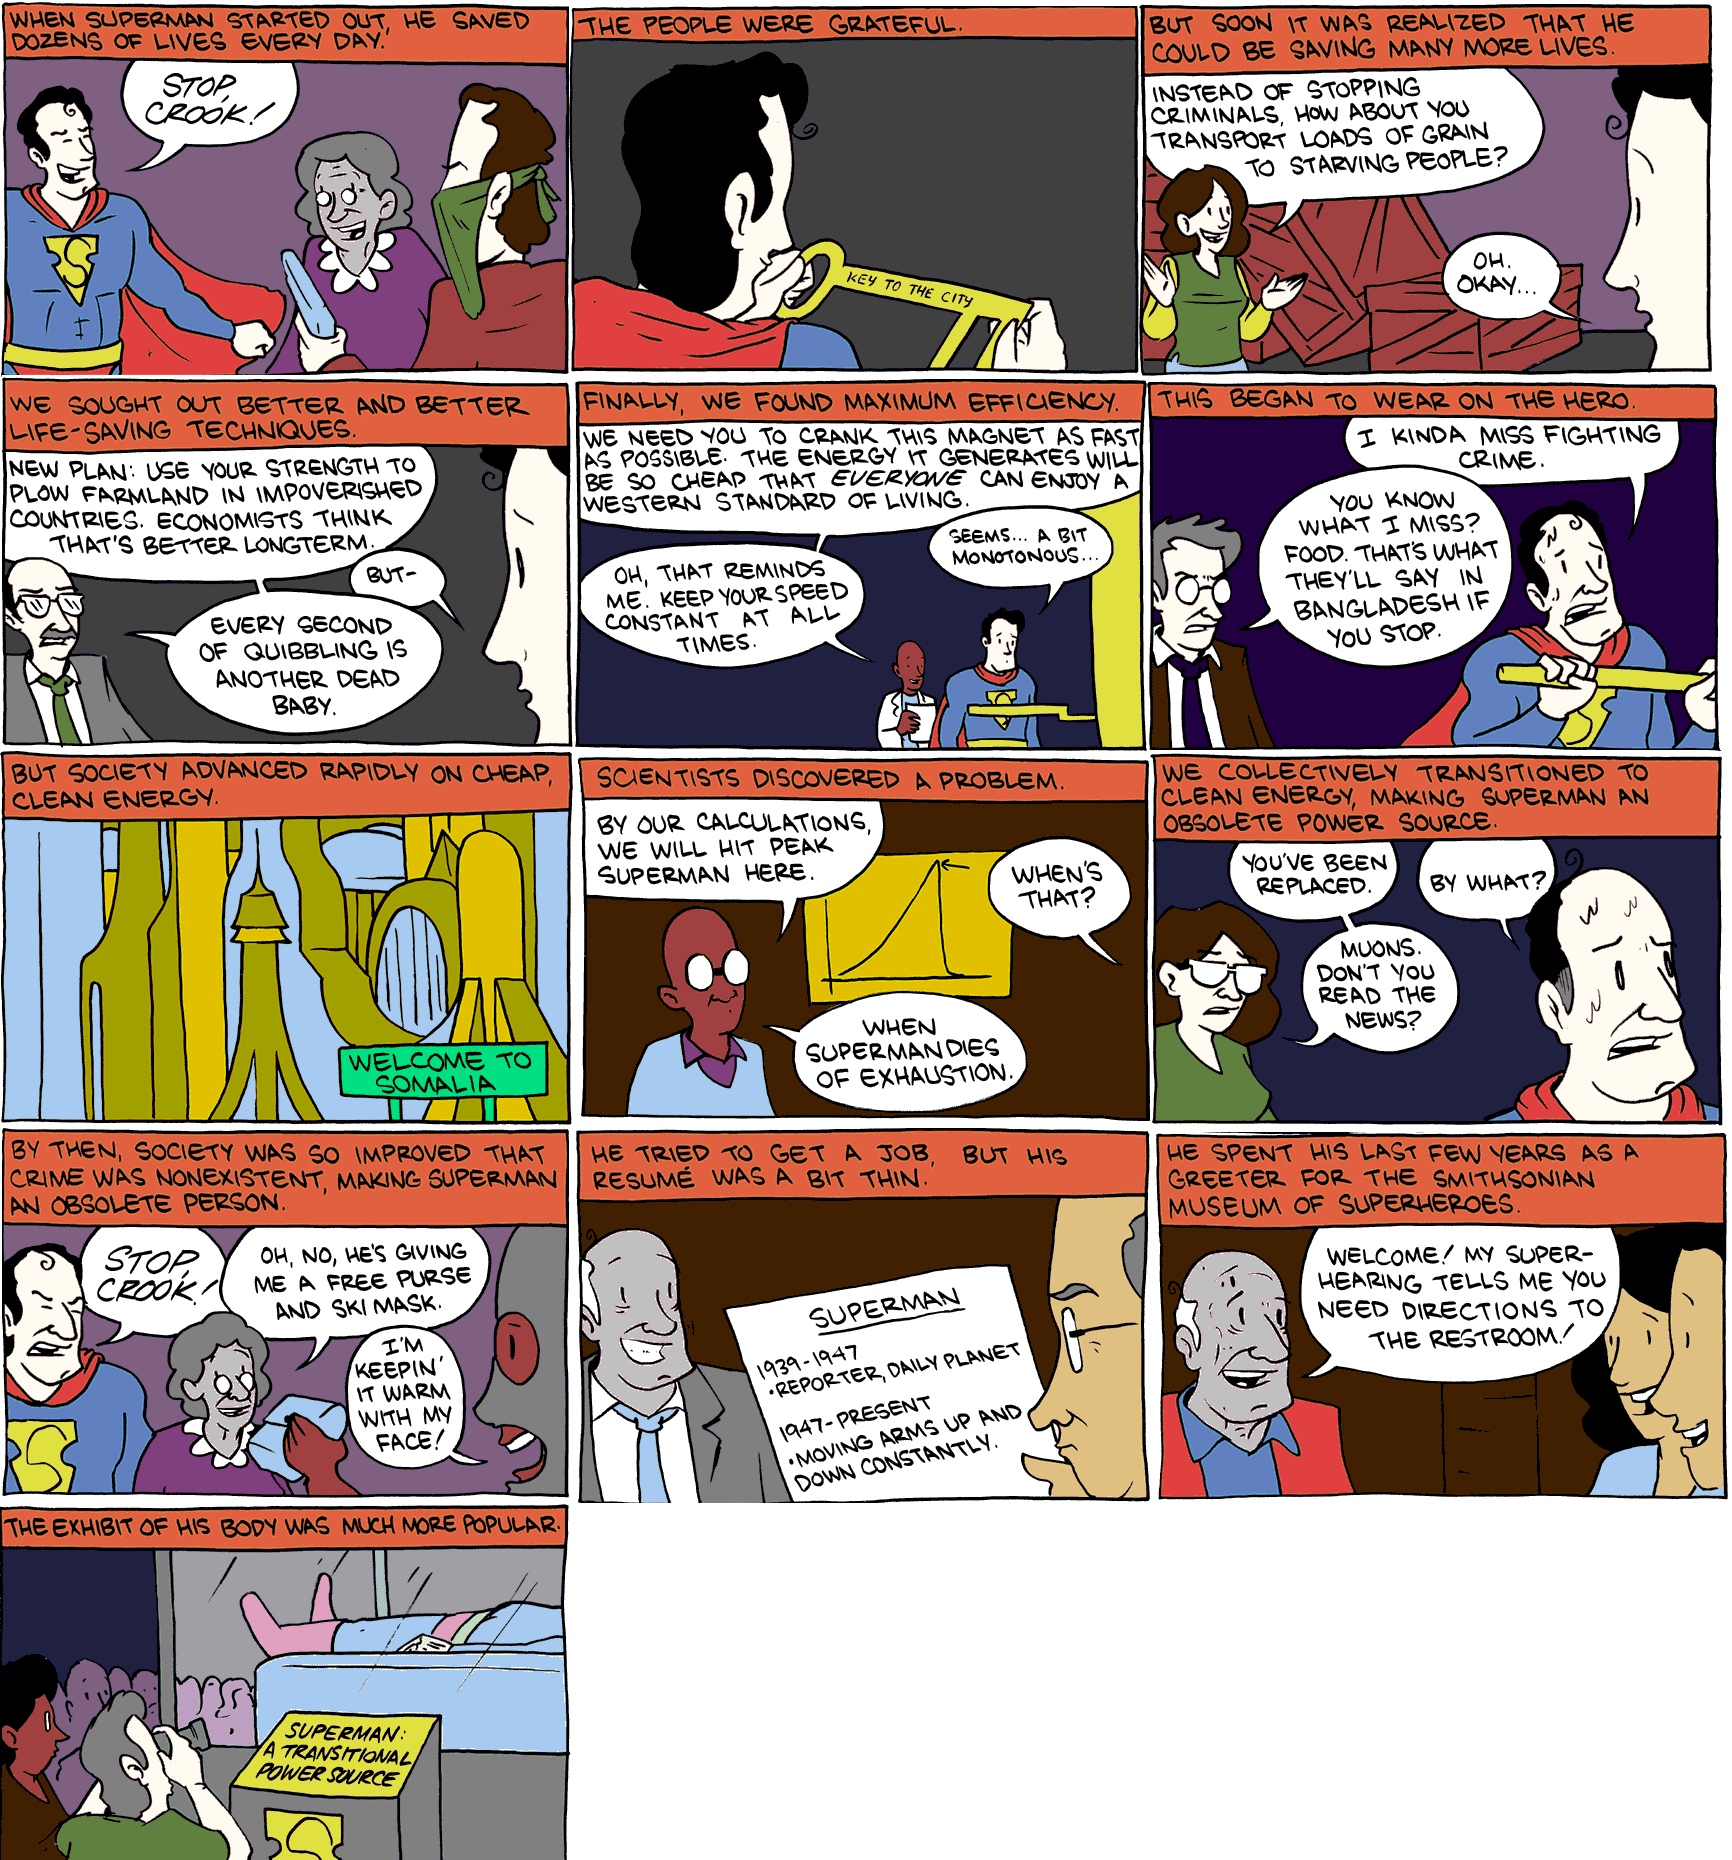
\includegraphics[width=\textwidth]{comic_superman}
	\caption{Super-homem como fonte de energia}
      \end{figure}
        
  \chapter{O Despertar dos Deuses e a Engenharia Contemporânea}

      Engenharia é “a capacidade de aplicar os conhecimentos científicos
      de forma prática a fim de produzir novas utilidades. Para obter tais
      resultados, o engenheiro estuda o problema, planeja uma solução,
      verifica a viabilidade econômica e por fim coordena o desenvolvimento
      ou produção”. Porém, hoje a utilidade também tem que ser sustentável.

  \chapter{O conceito das três partes}

    A ideia passada pelo texto de uma espécie dividida em três partes
    complementares, que precisam entrar em harmonia para completar o
    ser, incentivou uma análise da mente humana de forma similar. Esse
    conceito foi trabalhado por meio de comparações com o
    comportamento de pessoas reais de forma a maturar em um modelo no
    mínimo interessante que abre caminho para discussões filosóficas,
    sobre a necessidade da diversidade e os motivos de dissidências entre
    diferentes linhas de pensamento, por outra perspectiva. A ideia é
    descrita a seguir em tom de fenômeno físico observado mas não almeja
    ser tratado como um modelo da complexidade da mente humana. A
    termodinâmica é uma valida representação dos valores médios
    populacionais da mecânica estatística e a psicologia tentar fazer este
    papel em relação à neurologia. Da mesma, forma o modelo de três
    partes pode, talvez, representar bem as médias, sem qualquer
    conhecimento da complexidade humana.
    
    Dentro deste modelo, a mente fica dividida em três partes, chamadas
    de partes conservadora, dinâmica e racional. Um indivíduo pode nascer
    com uma destas partes melhor desenvolvida que as outras, e isso defineo seu modo de pensar, mas pode, e deve, desenvolver as três partes
    durante a sua vida. O desbalanceamento das três partes em um
    indivíduo, A, causa a incapacidade deste indivíduo compreender os
    pensamentos de outro indivíduo, B, que partem de uma das partes não
    desenvolvidas por A. Além da clara dificuldade de trabalhar em conjunto
    e respeitar outros pontos de vista, por considerar errados, um indivíduo
    A com uma das três partes mais desenvolvida do que as outras pode
    passar a não utilizar suas partes menos desenvolvidas por completo.

    \section{A analogia}
    
      Na segunda parte do livro “O Despertar dos Deuses”, “...os próprios
      deuses...”, o paternal, o emocional e o racional, de início tão
      desconectados e centrados em suas capacidades e modus operandi
      naturais, passam a se compreender cada vez mais, e, como
      consequência disso, não somente passam a atuar melhor em conjunto
      como também desenvolvem capacidades adicionais advindas do meio
      termo entre suas personalidades. Por fim estes entram em equilíbrio se
      tornando um só ser de capacidade maior do que a soma de suas
      capacidades individuais. Deste ponto principal da segunda parte do livro
      e da descrição das divergências de formas de pensar e agir dos três
      gêneros de “suaves”, o conceito do ser humano como uma composição
      de três “suaves” em desequilíbrio aparentemente explica as
      personalidades extremas e personalidades intermediarias encontradas
      pelo mundo, além de explicar suas convergências e divergências.
      
    \section{O conservador}
    
      O lado conservador está associado aos princípios básicos de
      sobrevivência de nosso ego. Diferente de racionalidade, um conjunto
      básico de regras imutáveis na forma de um “look-up table” tornam o
      sujeito majoritariamente conservador rápido e produtivo. Não existe
      muita margem para discussões ou mudanças, o conservador tem suas
      verdades bem definidas e uma memória longa, pouco “fator de
      esquecimento”, reforçando a primeira impressão sobre um assunto ou
      pessoa.
      
      Enquanto suas verdades não forem abaladas, o majoritariamente
      conservador é o mais confiável, por ser o mais previsível, e o mais
      produtivo, por não desviar de suas metas e conduta moral. O
      conservador não entra em discussões filosóficas sobre o sentido de sua
      vida, ele segue alguma crença divina ou senso moralista de justiça que é
      inabalável pela racionalidade alheia. Quando, de fato, o conservador
      perde sua crença, por se apoiar totalmente nela, ele fica completamente
      perdido.
      
      A associação desse comportamento com o funcionamento baseado
      em princípios básicos de sobrevivência é simples. Nossos instintos
      básicos são de cautela. Com memórias longas e enfáticas nas primeiras
      experiências, um animal não se aproxima de possíveis perigos e se
      preserva, mesmo quando desnecessariamente, mesmo quando não há
      um perigo real. “Better safe than sorrow”. Já o funcionamento por base
      em regras básicas e não por racionalidade é facilmente explicado pelo
      fato de que, na natureza, as vezes qualquer reação imediata vale mais
      do que uma reação pensada segundos depois. Correr para longe de um
      barulho repentino pode salvar a sua vida, enquanto tentar raciocinar se
      o barulho merece atenção ou não pode causar sua morte. Neste caso,
      correr a toa vale mais do que pensar se vale a pena correr. É claro que,
      da mesma forma que faço aqui, isto pode ser raciocinado previamente,porém, em uma situação repentina, dependeria do tipo da pessoa
      conseguir seguir o “script” ou tentar compreender a situação. O “medo”
      do desconhecido pode ser a reação certa a se ter, enquanto o indivíduo
      majoritariamente racional perderia tempo raciocinando sua reação no
      momento em que já deveria estar tomando alguma ação.
      
      Deve ser enfatizado que a característica principal do conservador é a
      auto preservação. Mudanças não são sempre evitadas apesar de sempre
      haver reclamação. Quando uma mudança acontece repentinamente, o
      reflexo do conservador é querer voltar para a situação anterior mesmo
      que isto seja impossível, pois nela ele sabe que sobrevive. Qualquer
      mudança subsequente que aproxime a situação atual à antiga será
      aceita e, depois, criticada. “Não está tão bom quanto antes”
      
      Fica aparente uma dicotomia entre o racional e o conservador neste
      quesito mas também existem uma dicotomias aparentes entre o
      dinâmico e o racional e entre o dinâmico e o conservador, mostrando o
      quão complementares estas ideias são. São estas aparentes dicotomias
      que criam os conflitos internos no indivíduo que tem dois “suaves”
      relativamente equilibrados mas a ausência do terceiro.
      
      O lado conservador se apresenta como um resquício evolutivo mas
      isso não justificaria uma maioria da população mundial
      majoritariamente conservadora, que de fato é o que pode ser
      constatado pensando melhor no assunto. Seria o mesmo que dizer que
      a população mundial está, em média, em sua infantilidade evolutiva.
      Esta situação pode ser melhor elaborada com a analogia à genética.
      
      \subsection{Analogia Genética}
      
	Pensando em seres mais primitivos, como bactérias unicelulares,
	vemos que seu código genético possui poucos mecanismos depreservação. Devido à isso, durante a replicação, muitas mutações
	acontecem causando grande diversidade. Para seres simples, isto pode
	ser visto majoritariamente como vantagem porém, para seres
	complexos e pluricelulares, isto pode fazer com que blocos funcionais,
	como o código para a mão ou o fígado, sejam modificados para algo não
	funcional. Para que isso não aconteça, foi necessário o desenvolvimento
	de formas mais conservadoras de replicação genica, com verificação e
	correção do código após replicação e modificações feitas por troca de
	blocos funcionais inteiros entre diferentes alelos, “crossing-over”, de
	forma a manter a evolução, porem de forma menos dinâmica
	preservando blocos funcionais.
	
	Da mesma forma, uma população que não fosse majoritariamente
	conservadora implicaria numa grande massa de pensamento
	divergente, causando revoluções constantes, não necessariamente para
	melhor, reduzindo a produtividade total. Se todos estão preocupados
	em criar novas ferramentas para o plantio, ninguém está plantando
	nada e todos vão morrer de fome. Se muitos gastam o dia discutindo
	sobre quais religiões estão erradas, os conservadores que tem lastro
	nessas religiões perdem produtividade por influência da inserção de
	dúvidas, enquanto os que discutem em si não produzem nada.
	
    \section{O dinâmico}
      
      Ao contrário do conservador, o dinâmico não utiliza nenhum tipo de
      lastro e não se apoia em memória. Está constantemente buscando
      modificações e sempre insatisfeito. Este lado é baseado em nossa
      necessidade de evoluir. Assim como em algoritmos genéticos, na
      verdade exatamente como, todos os humanos dão saltos randômicos de
      opinião e forma de pensar. Estas são questionadas e pontuados, claroque essa pontuação só será eficiente com o desenvolvimento racional,
      e novos passos são dados de forma a encontrar ótimos locais. O princípio
      do “suave” dinâmico é o que impede que o ser convirja em máximos
      locais. É a “mutação” no algoritmo genético que impede que se convirja
      em um máximo local, possibilitando que se alcance o máximo global.
      Esse papel aleatório deve ser o princípio da criatividade. Fica claro de
      antemão que a calibração das três partes em uma população deve
      funcionar analogamente a calibração de um algoritmo genético.
      
      O majoritariamente dinâmico acaba sendo um indivíduo
      improdutivo, que passa seus dias filosofando sobre tudo, invés de
      produzindo algo, mas sem a racionalidade necessária para chegar a
      conclusões. Instável e de difícil convivência, normalmente não é
      respeitado pelos majoritariamente conservadores por serem inúteis
      nem pelos majoritariamente racionais por serem irracionais.
      
      Vendo que o cérebro humano processa mais informação do que o
      ego tem consciência de, podemos conjecturar a possibilidade de utilizar
      esta informação. Isto poderia justificar a sensação de estar sendo
      observado de uma direção fora do seu campo de visão. O
      processamento paralelo de toda a informação de todos os sensores do
      corpo humano pode acionar alarmes para nosso ego sem que as
      informações necessárias para chegar nestas conclusões sejam todas
      entregues. O dinâmico desenvolve seu lado intuitivo e talvez se torne
      mais receptivo aos “alarmes” do cérebro. Isto possibilitaria tomar uma
      decisão correta sem ter a capacidade de compreender a situação por
      completo. Como o teorema de Gödel mostra que um sistema só
      consegue compreender outro sistema mais simples que ele mesmo, e
      existem muitos sistemas mais complexos que o sistema racional quecompõe o ego, o “suave” dinâmico contornaria este problema
      recebendo informações do sistema neural completo, além do ego.
      
      O processamento linear e sequencial da racionalidade matemática
      possui limites pelo seu sistema inerente, o ego humano, enquanto o
      sistema neural completo, com processamento paralelo, ultrapassa a
      linha racional de pensamento. A compreensão sem compreender é
      marca deste tipo dinâmico, que “sente” a resposta ao invés de raciocina-
      la. Apesar de parecer uma característica artística mais do que científica,
      parece ser o diferencial de homens como Einstein ou Newton, que
      conjecturavam ideias corretas sobre o universo mesmo que contra
      intuitivas ao racionalismo aplicado ao conhecimento da época. De fato,
      o estado-da-arte apresenta uma característica de “feeling” que pouco
      pode ser descrita como resultado de pensamento matemático linear
      racional.
      
      Mesmo tentando explicar este “sentimento” em cima das
      informações, o funcionamento do “suave” dinâmico parece exceder a
      simples utilização da habilidade inerente do cérebro de processamento
      paralelo, assim como é difícil de caracterizar a criatividade por algo não
      estocástico. Talvez seja a falta de conservadorismo que possibilite que
      fleches de ideias, que surgem randomicamente em nossas mentes, se
      propaguem o suficiente para se tornar um conceito trabalhado. As vezes
      isso pode gerar ideias descartáveis e erradas mas também pode levar a
      verdades contra intuitivas.
    
    \section{O racional}
      
      Apesar de parecer auto explicativo e absolutamente positivo, o
      racional possui o defeito de ser racional. Devido aos desenvolvimento
      de Gödel, ficou demonstrado que existe um limite para a compreensãodo universo por parte de um integrante deste universo. Somente pode
      ser compreendido algo de complexidade menor que o sistema que tenta
      o compreender. A ideia de que tudo pode ser compreendido e
      racionalizado está errada e um indivíduo que não consegue contornar
      algo incompreensível pode ficar preso em paradoxos. Além disso, no
      mundo prático, não ter reações na forma de “look-up table” não é
      eficiente em muitos casos, como foi discutido sobre o conservador.
      
      Entre um “suave” puro de cada tipo, o racional ainda é o melhor
      opção como líder.
      
    \section{Psicologia Social}
    
      No âmbito da psicologia social, o modelo das três partes pode
      explicar a “foot-in-the-door technique”, onde, ao se pedir cada vez mais,
      aos poucos, pode-se convencer alguém a algo que não seria possível
      pedindo de uma só vez. Como nenhum indivíduo é puramente
      conservador, sempre é possível lhe convencer à algo ligeiramente além
      do seu comum, desde que não saia muito de suas verdades primárias. O
      estado atual desde indivíduo passa a ser o de quem aceita, também, está
      nova condição. Com o seu “look-up table” atualizado, agora, o processo
      pode ser repetido. Um indivíduo puramente conservador não teria
      aceitado nenhuma forma de persuasão para fora de seu modus
      operandi. No entanto, um majoritariamente conservador permitiria esta
      flexibilidade e, ao mesmo tempo, se basearia em comparar suas
      premissas atuais com o que está sendo pedido para decidir aceitar ou
      não. Isto permite a “foot-in-the-door technique”. Com um indivíduo
      majoritariamente racional ou dinâmico o mesmo não acontece, o
      primeiro por só ser persuadido por razão e o segundo por decidir de
      forma aleatória, na média seria meio a meio de sim e nãos, ou porsentimento, o que não seguiria uma cadeia de aceitações baseadas nas
      aceitações anteriores.
      
      Também pode-se explicar casos como o terceiro Reich e o massacre
      de Ruanda pela maioria ser majoritariamente conservadora, como
      citado previamente. Casos em que as pessoas são levados ao extremo
      aos poucos são possíveis, novamente, pelo conservadorismo que
      enfatiza a situação encontrada mais do que a mudança. O racionalismo
      por outro lado, independente da cultura e situação local, discerne o
      construtivo do destrutivo. Para alguns falta a racionalidade para
      compreender as interconexões existentes entre os indivíduos e entre a
      natureza como um todo, fazendo que estes ajam de forma não
      construtiva e egocêntrica, enquanto em outros o sentimento da ação
      coletiva prevalece mesmo sem uma lógica. Em outros casos, o
      sentimento de interconexão faz com que uma ação seja rejeitada por
      parecer egocêntrica quando na verdade é a melhor ação para o coletivo.
      A inercia social que o conservadorismo causa impede mudanças bruscas
      mas não impede mudanças gradativas. Ao mesmo tempo, impede que
      mude-se a direção em que a sociedade se move, mesmo que em direção
      a um abismo. Em situações de crise e falta de lastro, o conservador é
      levado ao extremo e, ao encontrar uma ideia para se lastrear, fica preso
      e molda sua realidade em cima dela. Após observar resultados positivos
      da política externa do terceiro Reich para a Alemanha, o povo assumiu
      o Reich como sua religião.
      
  \chapter{Conclusão}

   Asimov nos convida a refletir sobre o papel da humanidade e o balanço entre energia farta e barata ao custo do desconhecido, 
   contra o status quo. Basicamente é uma viagem ao interior do psique humana, que é expressa metaforicamente pelos para-seres que 
   denotam as diversas facetas do ser humano em seres distintos. 

   Os paralelos com a carreira na área de engenharia são diversas, dentre elas são citadas as responsabilidades inerentes das aplicações 
   de novas tecnologias, metodologias ou qualquer outra dinâmica que afete a humanidade como um todo. Hoje, por exemplo, muito se fala em 
   energia renovável e só a prudência e o incansável questionamento, erros e acertos das carreiras científicas, engenharias inclusas, dirão 
   o quão renováveis e sustentáveis realmente são. 

   Portanto podemos atribuir à carreira na área de engenharia não só o prestígio, mas a responsabilidade que advém do conhecimento para transformar o mundo.
   
\end{document}
